\documentclass{article}
\usepackage{graphicx} % Required for inserting images

\title{statistics group project- Explanation of american tire industry decline in the 21st century on the divergence in domestic and foreign prices for tires}
\author{Michal Stránský, Lukáš Doležal, Jakub Černý}

\begin{document}

\maketitle
\subsection*{Content}
Why tire industry is in such decline\\
    equity low prices\\
    decline compared to aggregate us - histogram? 
histogram of top countries importing? \\
explanation\\
    boxplot of wages\\
    scatterplot\\
        price compared to volumes of industry\\
        any correlation?\\
        
\subsection*{Abbrevations}
BLS - bureau of Labor statistics , HS - harmonized system, NAICS - North American Industry Classification System, FRED - Federal Reserve Economic Data
\section{Introduction}
Open 1 or 2 sentences about motivation\\
\textbf{Requst:}\\

\textbf{Sources of data}\\
Write please the sources so we dont forget about them later\\
We primarly used data from american government agencies: 
		centered{ census.gov for hs imports data, fred - to recover BLS data (except for CPI), BLS to retrieve CPI data, 
		FROM BLS we retrieved data from PPI, CPI and productivity surveys.
\section{rozd2len9 prace}

vse od roku 2000
U FRED pozor na seasonal adjusted
!!!NESTAHOVAT EXCEL, ALE CVS!!!
lukAS - mean, median (nonDURABLE GOODS - FRED)
lukas - histogram, porovani objemu produkce u 40 statu (najit 100) 2025
Michal - scatterplot domaci cena/venkovni cena 

korelace
cena (domacich)/zaharnicnich pneumatik, vuci volume
\section{Development of tire production in the US }
% 'Pak ty grafy jeste pozdeji upravim + zejtra pridam ten oddil k histogramum
As illustrated in Figure \ref{fig:figure1}, U.S. domestic tire production was largely stagnant at the beginning of the 21st century. Production began at a level of 127.5 and ended at 124.3 (the year 2017 serves as the base year) by the third quarter of 2007. Between 2008 and 2010, production experienced a sharp decline up to 20 percentage points, as demonstrated in Figure \ref{fig:figure2}. Although production initially saw a dramatic recovery in 2010, it quickly returned to a state of stagnation. Subsequently, the COVID-19 Pandemic triggered another severe contraction, with production dropping by more than 20 percent, though it rebounded by roughly 20 percent shortly after. Following this recovery, production began to stagnate and eventually started contracting even more. By the fourth quarter of 2020, the production level stood at 99.8, representing a slight decrease from Q4 2019, and ultimately fell to 72.8 by Q1 2026. 
\begin{figure}[htbp]
    \centering
    \begin{minipage}{0.7\textwidth}
        \centering
        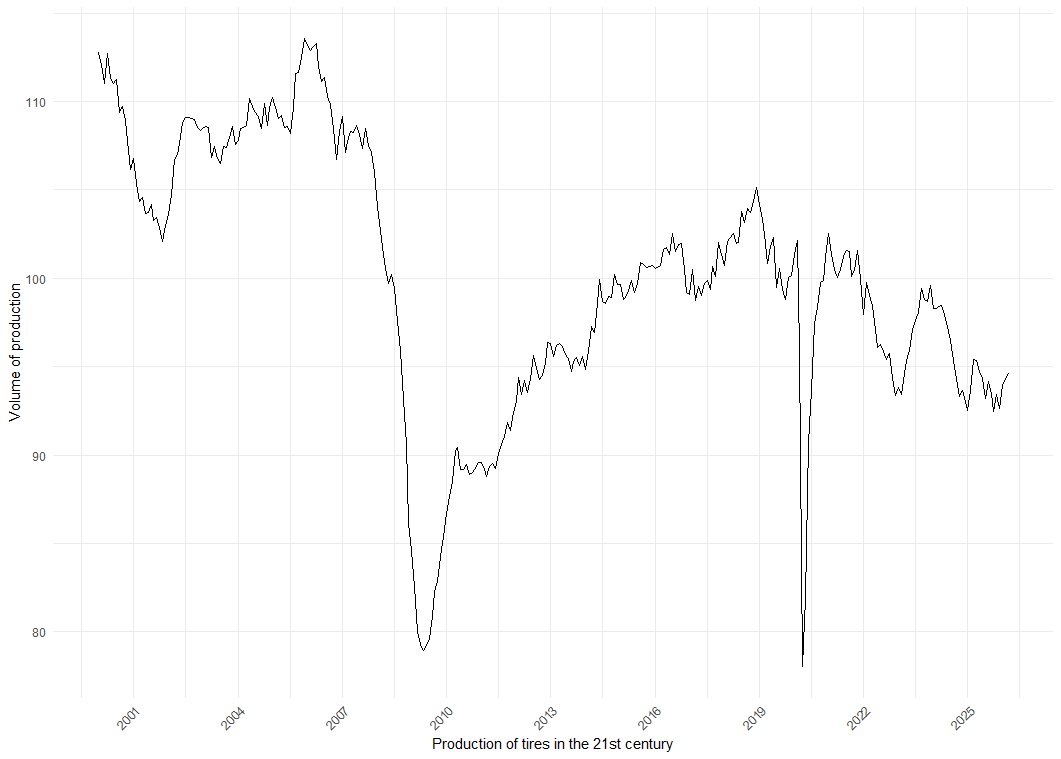
\includegraphics[width=\linewidth]{images/timeseries_productionvolume.png}
        \label{fig:figure1}
    \end{minipage}\hfill 
    \begin{minipage}{0.7\textwidth}
        \centering
        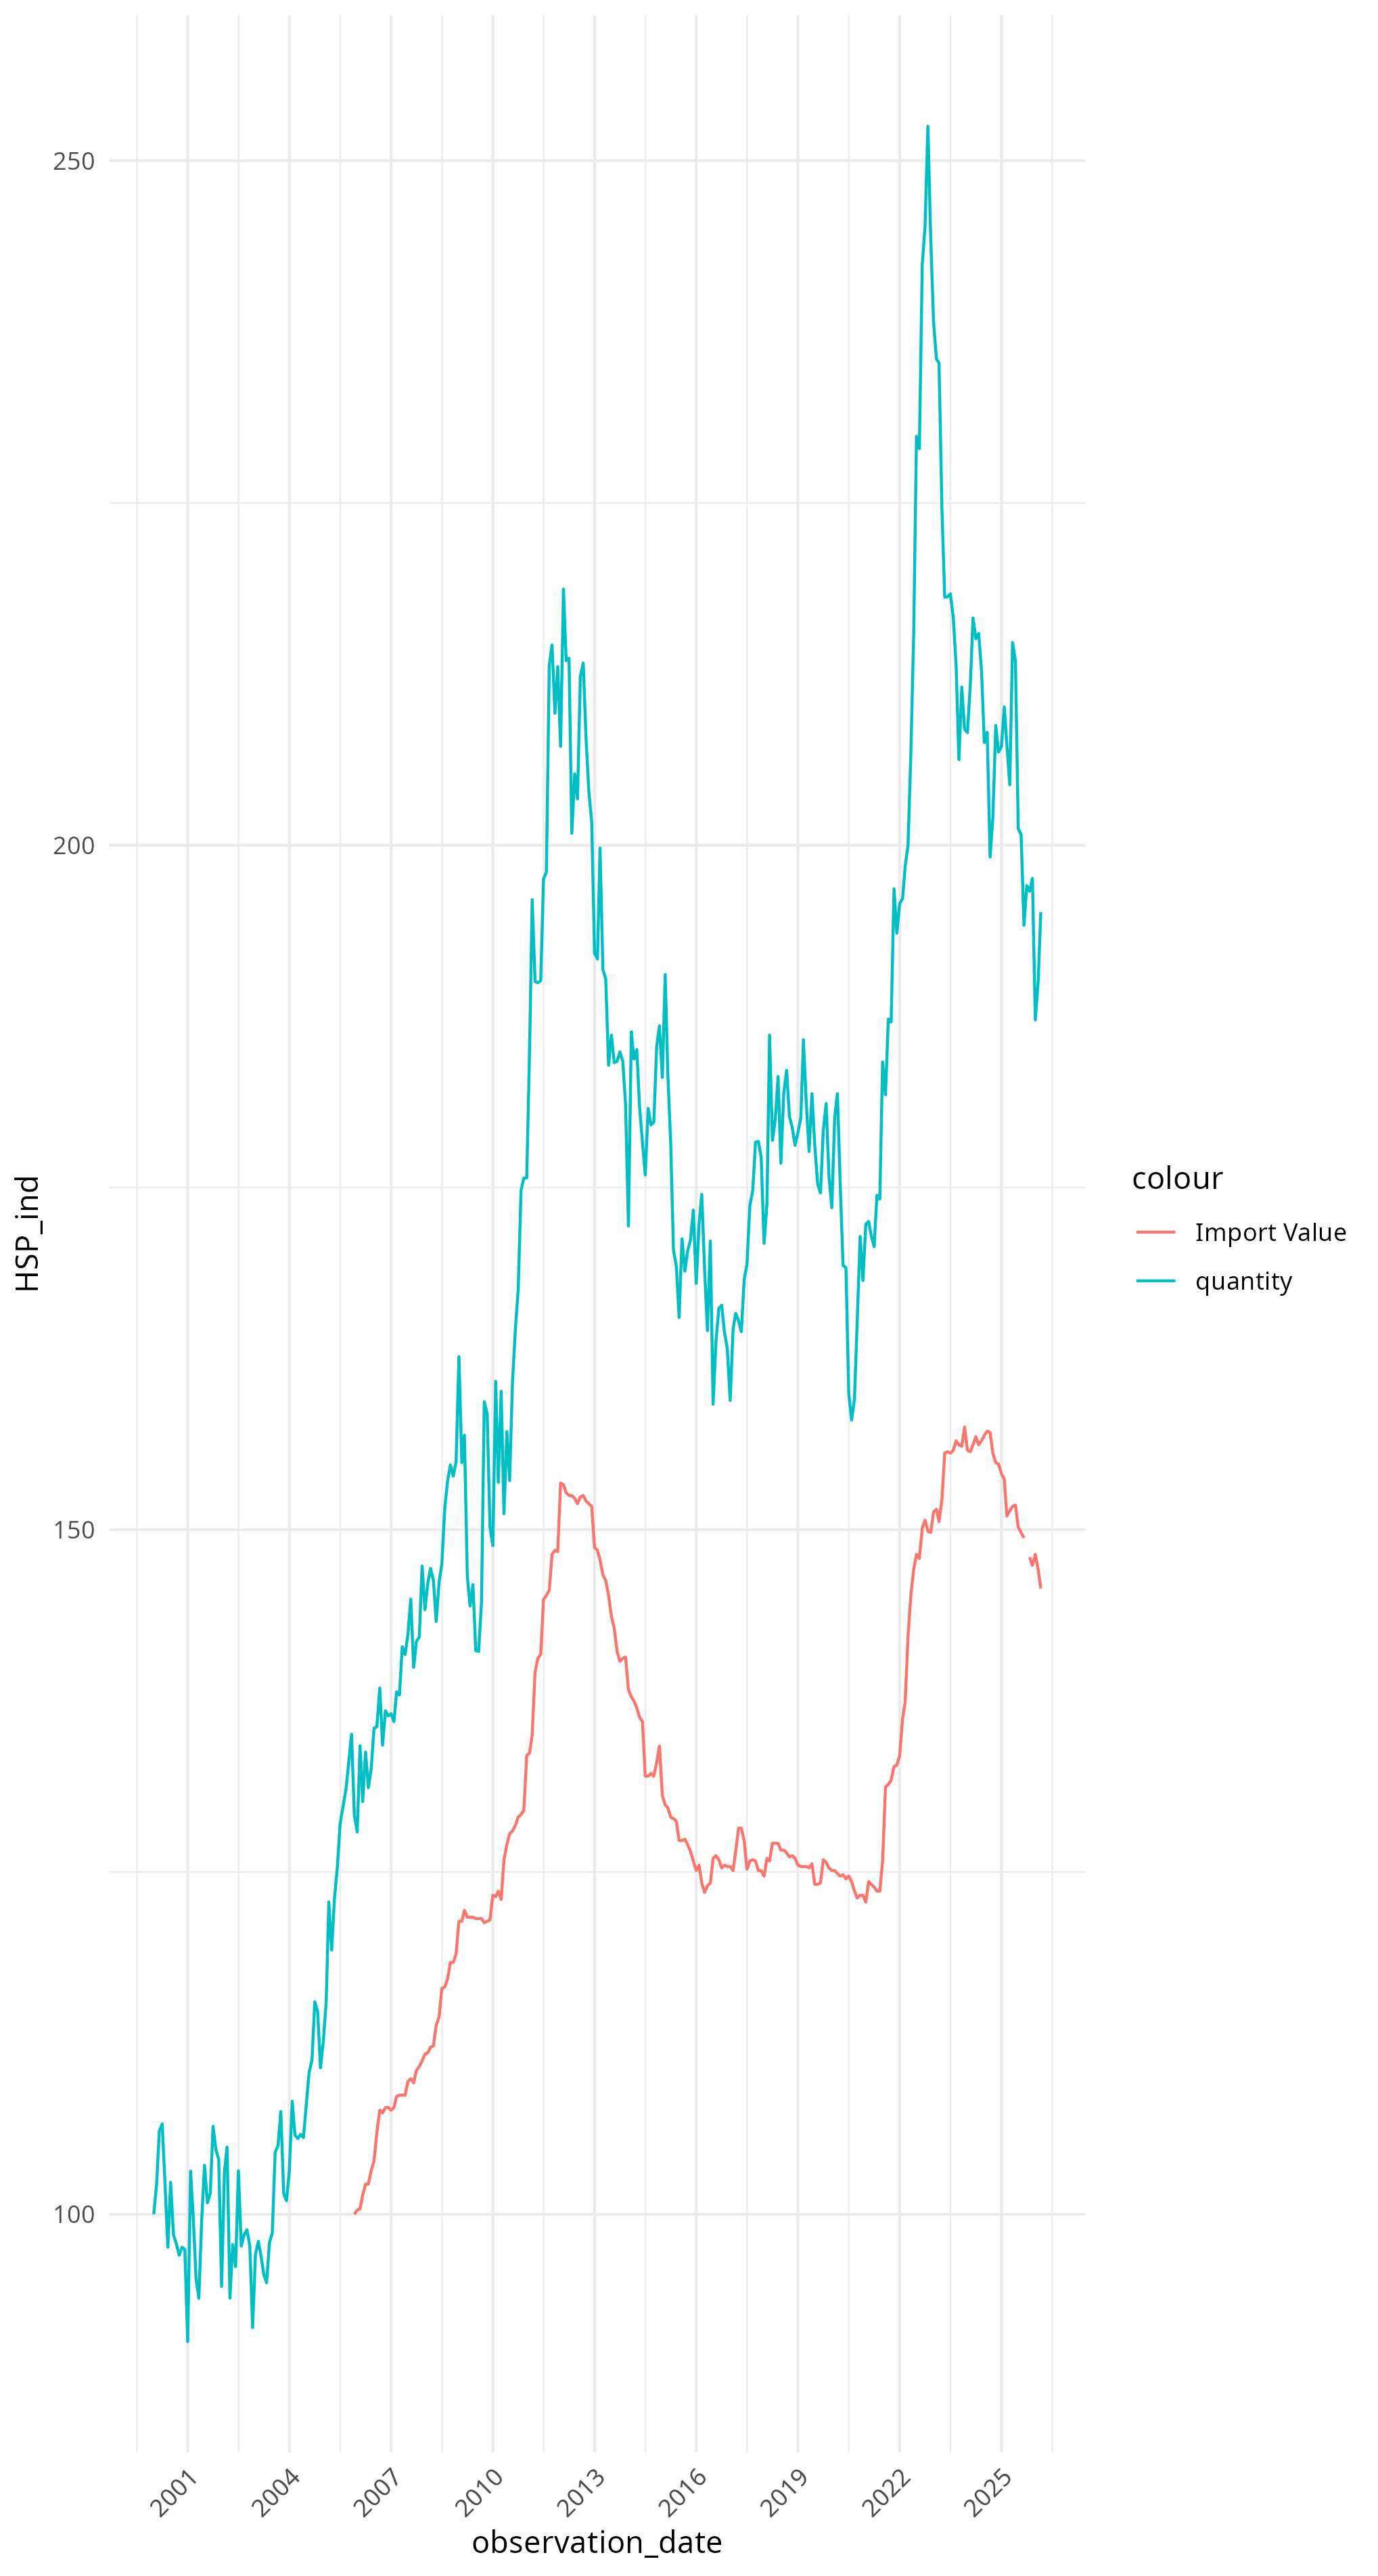
\includegraphics[width=\linewidth]{images/timeseries_growthrates.png}
        \label{fig:figure2}
    \end{minipage}
\end{figure}

As seen in \ref{fig:figure3},\ref{fig:figure4} and \ref{fig:figure5}, the US is in the sixth place in the world in exports, while five years later it is not in the top ten tire exporting countries, the country is instead in 12th place. And four years later in 2024 the US has fallen to 16th place. The export position of the US was consistently falling. In 2015, 2020 and 2024 China and the EU are positioned in the first place, and the second place respectively in exporting tires.
\begin{figure}[htbp]
    \centering
    \begin{minipage}{0.7\textwidth}
        \centering
        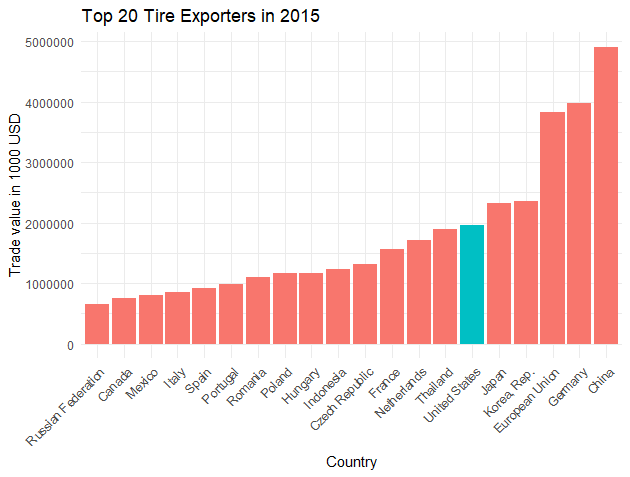
\includegraphics[width=\linewidth]{images/top20exporters_2015.png}
        \label{fig:figure3}
    \end{minipage}\hfill 
    \begin{minipage}{0.7\textwidth}
        \centering
        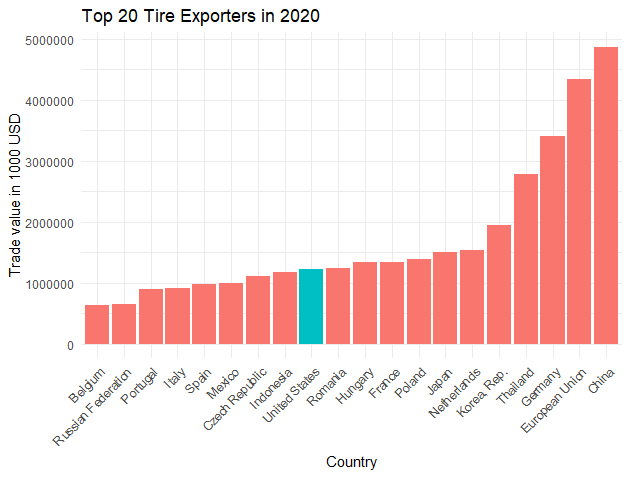
\includegraphics[width=\linewidth]{images/Top20tireExporters_2020.png}
        \label{fig:figure4}
    \end{minipage}
    \begin{minipage}{0.7\textwidth}
        \centering
        \includegraphics[width=\linewidth]{images/Top20Exporters_2024.png}
        \label{fig:figure5}
    \end{minipage}
\end{figure}


The median growth rate stands at 0.43 percent and a mean at -0.58 percent. The maximum and minimum growth values were recorded at 22.04 percent in Q2 2021 and -22.82 percent in Q2 2020, respectively. The standard deviation of growth rates is 5.89 and for volumes of production stands at nearly 7.48. The median growth of the total US industrial production is nearly 1.63 and the mean is 0.58 percentage points. In comparison to the tire industry growth both values are higher. Although the maximum rate of growth was lower at 16.55 percent in 2021 in comparison to the tire industry, but the minimum value is larger as it stands at -17.31 in 2020. Both largest recoveries and slumps occurred in the same period during COVID-19 Pandemic.

Furthermore, the accompanying boxplot, which is \ref{fig:figure7}, indicates that the distribution of growth rates is rather left-skewed. This skewness is supported by the fact that the mean is being lower than the median. It is also notable that the majority of outliers fall below the mean, suggesting that the industry experienced a greater frequency of sharp declines compared to sudden recoveries. Prominent examples of these outliers include the drastic drop during the aforementioned COVID-19 pandemic, as well as the subsequent recovery phase in 2021.
\begin{figure}[htbp]
    \centering
    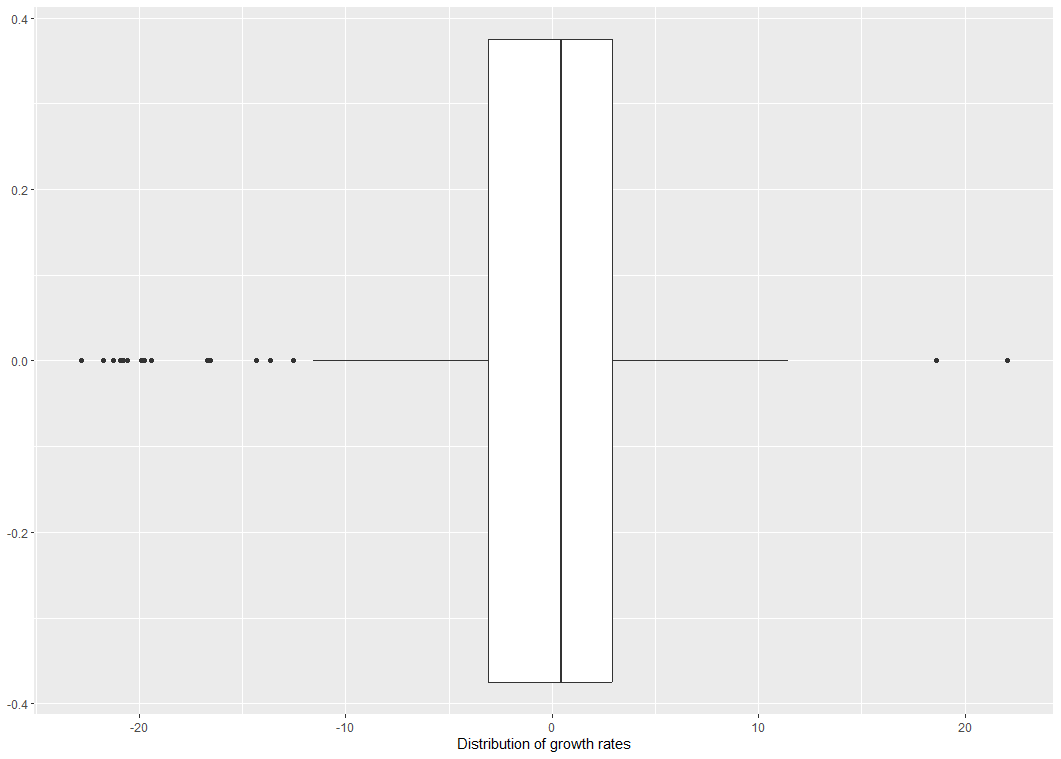
\includegraphics[width=0.5\textwidth]{images/boxplot.png}
    \label{fig:figure6}
\end{figure}

\section{ty zeme + jeste nejak vymyslim ten histogram}
As seen in \ref{fig:figure7}, which is a histogram, the volumes of exports of most countries are located near zero, the export market is dominated by states such as People’s Republic of China, the European Union, Thailand, etc.
\begin{figure}[htbp]
    \centering
    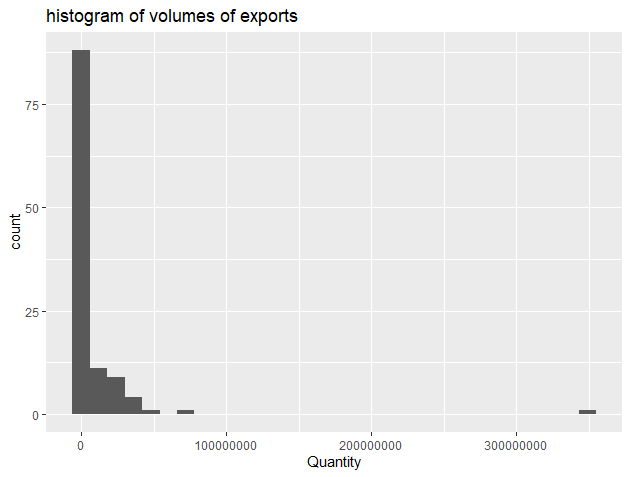
\includegraphics[width=0.7\textwidth]{images/histogramofvolumesofexports.png}
    \label{fig:figure7}
\end{figure}

The \ref{fig:figure8} gives a better picture of the distribution as
\begin{figure}[htbp]
    \centering
    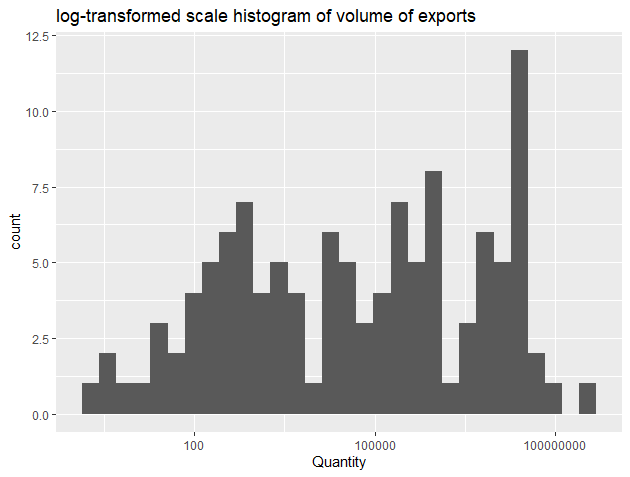
\includegraphics[width=0.7\textwidth]{images/loghistogramofexports.png}
    \label{fig:figure8}
\end{figure}
\end{document}